%Projekt c.5
%Autor: Ján Jusko
%Dátum: 7.5.2014

\documentclass[fyma2,pdf,final]{prosper}

\usepackage[czech]{babel}
\usepackage[utf8]{inputenc}
\usepackage[T1]{fontenc}
\usepackage{picture}
\usepackage{graphicx}

\slideCaption{\textit{Typografie}}
\DefaultTransition{Wipe}

\begin{document}

\providecommand{\uv}[1]{\quotedblbase #1\textquotedblleft}

%---------------------------------------------------
%\slideCaption{ITY -- proj5}
\title{Typografie}
\subtitle{Projekt č. 5 do předmětu ITY}
\author{Ján Jusko}
\institution{Vysoké učení technické v~Brně\\Fakulta informačních technologií}

\maketitle

%---------------------------------------------------
\begin{slide}{Úvod do typografie}
\begin{itemize}
	\item Dějiny typografie ve vlastním slova smyslu začínají, když Johannes Gutenberg v roce 1448 vynalezl knihtisk.\medskip
	\item Pojem typografie pochází ze spojení řeckých slov typos \uv{forma} a graphien \uv{psát}. \medskip
	\item Typografie se zabývá problematikou grafické úpravy tištěných dokumentů s použitím vhodných řezů písma a uspořádání jednotlivých znaků
 a odstavců ve vhodné, pro čtenáře srozumitelné a esteticky přijatelné formě.\medskip	
\end{itemize}
\end{slide}
%---------------------------------------------------
\overlays{5}{
\begin{slide}{Historie}
	
    \fromSlide{2}{
	\begin{itemize}
		\item V minulosti byla typografie uznávaná vědná disciplína. \medskip
	\end{itemize}}
	
    \fromSlide{3}{    
	\begin{itemize}
		\item Tištených dokumentů nebylo moc, proto se dbalo na jejích kvalitu.\medskip
	\end{itemize}}
	
    \fromSlide{4}{
		\begin{itemize}
        \item S rozmachem knihtisku přibývali i nové rodiny písma.\medskip
		\end{itemize}}

    \fromSlide{5}{
	\begin{itemize}
        \item Do různorodosti typografie přispěl významným dílem angličan \linebreak \emph{William Caslon *1693 \,--\, \textdagger 1766.}
	\end{itemize}}
\end{slide}
}
%---------------------------------------------------
\begin{slide}{William Caslon}

\begin{center}
		 \begin{figure}
             \scalebox{0.7}{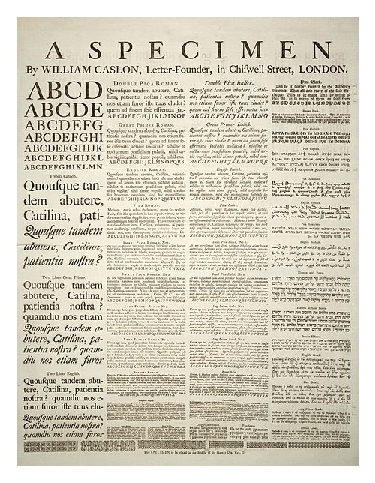
\includegraphics{specimen.eps}}
			\caption{Ukázka jeho práce z roku 1728.}
		 \end{figure}
        \end{center}
\end{slide}
%---------------------------------------------------
\overlays{6}{
\begin{slide}{Současnost}
	
    \fromSlide{2}{
	\begin{itemize}
		\item V dnešní době se pod pojmem typografie rozumí hlavně sázení elektronických dokumentů, webových stránek nebo časopisů. \medskip
	\end{itemize}}
	
    \fromSlide{3}{    
	\begin{itemize}
		\item Sází se výhradně na počítači.\medskip
	\end{itemize}}
	
    \fromSlide{4}{
		\begin{itemize}
        \item Na typografickou stránku dokumentů se neklade takový důraz.\medskip
		\end{itemize}}

    \fromSlide{5}{
	\begin{itemize}
        \item I přesto se dnes najde mnoho příznivců typografie.\medskip
	\end{itemize}}
	
	\fromSlide{6}{
	\begin{itemize}
		\item V České republice se vydáva časopis TYPO zaměřený na typografiu a vizuální komunikaci.
	\end{itemize}}
	
\end{slide}
}
%-------------------------------------------------
\begin{slide}{Časopis TYPO}

\begin{center}
		 \begin{figure}
             \scalebox{0.4}{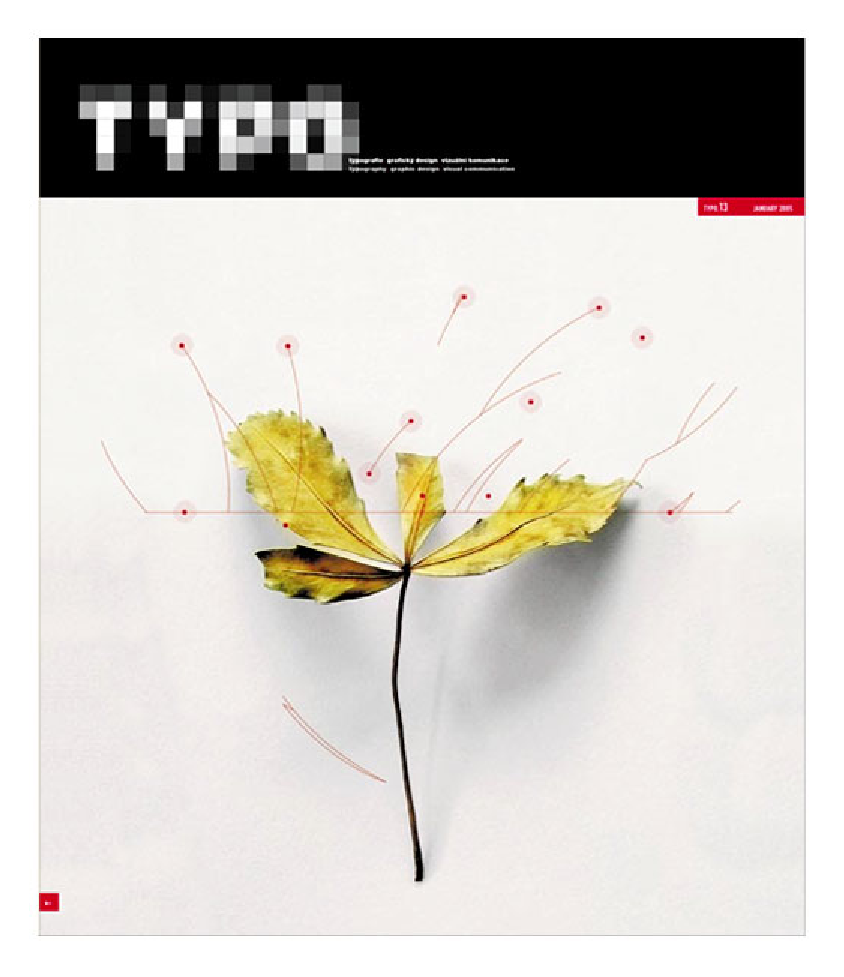
\includegraphics{casopis.eps}}
			\tiny{\caption{Ukázka časopisu TYPO.}}
		 \end{figure}
        \end{center}
\end{slide}

%---------------------------------------------------
\begin{slide}{Použité zdroje}
\begin{itemize}
		\item http://tvorim.net/typografia
\end{itemize}
\end{slide}
%---------------------------------------------------
\begin{slide}{}
\vspace{42pt}
%\vspace{\stretch{0.42}}
\begin{center}
{\large Děkuji za pozornost}
\end{center}
\end{slide}

\end{document}
